\documentclass[11pt]{article}

\usepackage{fullpage} % Use the full page
\usepackage{color}
\usepackage{tikz}
\usepackage{matlab-prettifier} % Matlab
\setlength\parindent{0pt} % No indentation


% Headers
\usepackage{fancyhdr}
\setlength{\headheight}{15.2pt}
\pagestyle{fancy}
\setlength\headsep{30pt}
\lhead{Youssef Beltagy and Samuel Hunter}   					%  Your name on the left header.
\chead{\textsc{Lab 2}}			%  Title in the center.
\rhead{\today}							%  Date on the right header.

% Matlab blocks
\lstset{
  style              = Matlab-editor,
  basicstyle         = \mlttfamily,
  mlshowsectionrules = true,
  escapeinside={//}{\^^M},
}

% Cover Page Settings
\title{
    \textsc{Lab 2 Report: Nonlinear Systems, Filters, and Convolution}
}

\author{
    \Large{Youssef Beltagy and Samuel Hunter} \\
    \large \textsc{AUT21 BEE 235}
}

\date{\today}



%--------------------------------------------
%%%%%%%%%%%%%%%%%%%%%%%%%%%%%%%%%%%%%%%%%%%%%%%%%%%%
% END OF THE PREAMBLE AND BEGINNING OF THE ACTUAL DOCUMENT
%%%%%%%%%%%%%%%%%%%%%%%%%%%%%%%%%%%%%%%%%%%%%%%%%%%%
%--------------------------------------------

\begin{document}


\maketitle % Make the cover page
\pagebreak


\section{Abstract}

In Part 1, the lab introduced concepts of implementing rectifiers and filters.
It then combined a rectifier with a low-pass filter to extract the enveloope of an audio signal.

\section{Part 1 --- Nonlinear rectifier and envelope extraction}

\subsection{Exercise 1}

\lstinputlisting{graph_rectifiers.m}

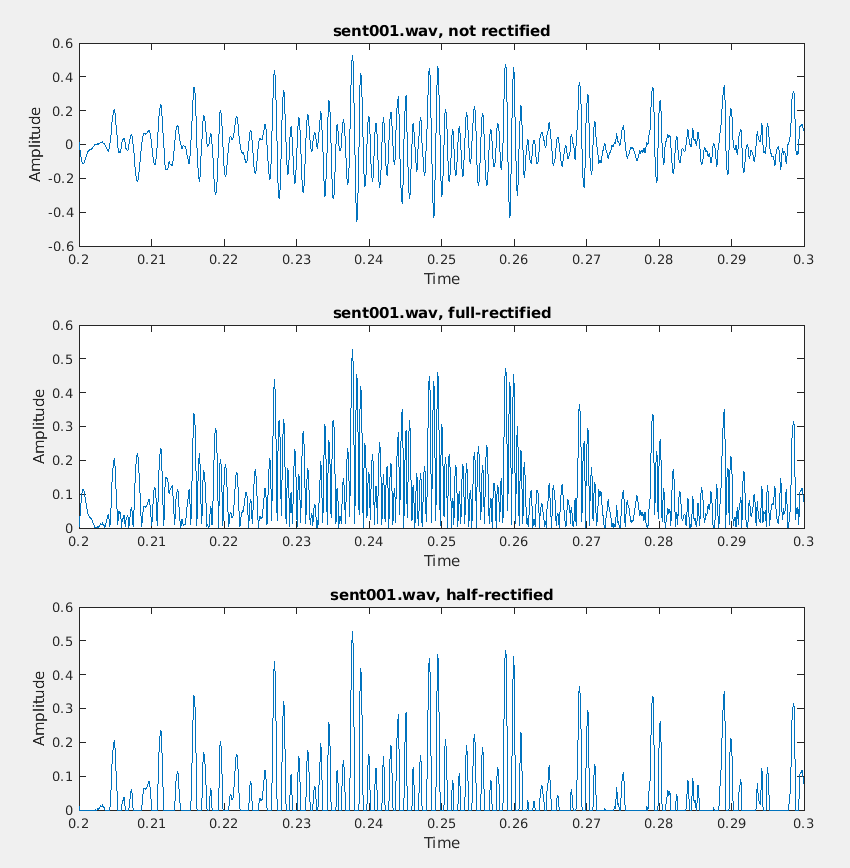
\includegraphics[width=\textwidth]{exercise1.png}

\subsection{Exercise 2}

After running \textit{sent001.wav} through the 500 Hz low-pass filter, the audio gave a distorted, coming-from-another-room sound:

\lstinputlisting{low_pass_filter.m}

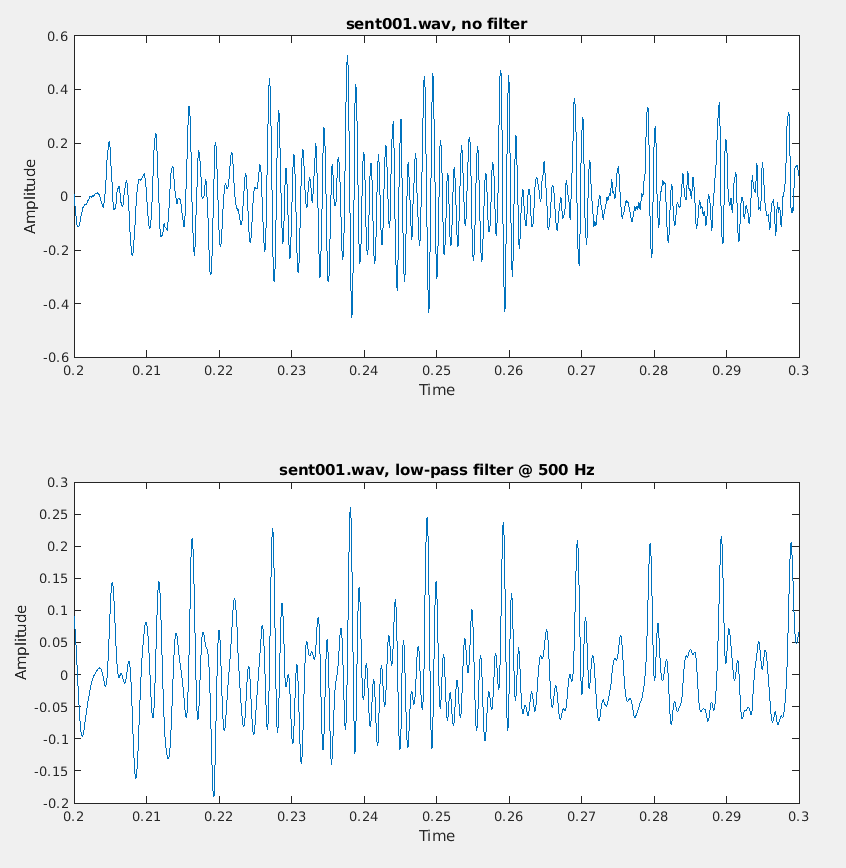
\includegraphics[width=\textwidth]{exercise2.png}

\subsection{Exercise 3}

\lstinputlisting{high_pass_filter.m}

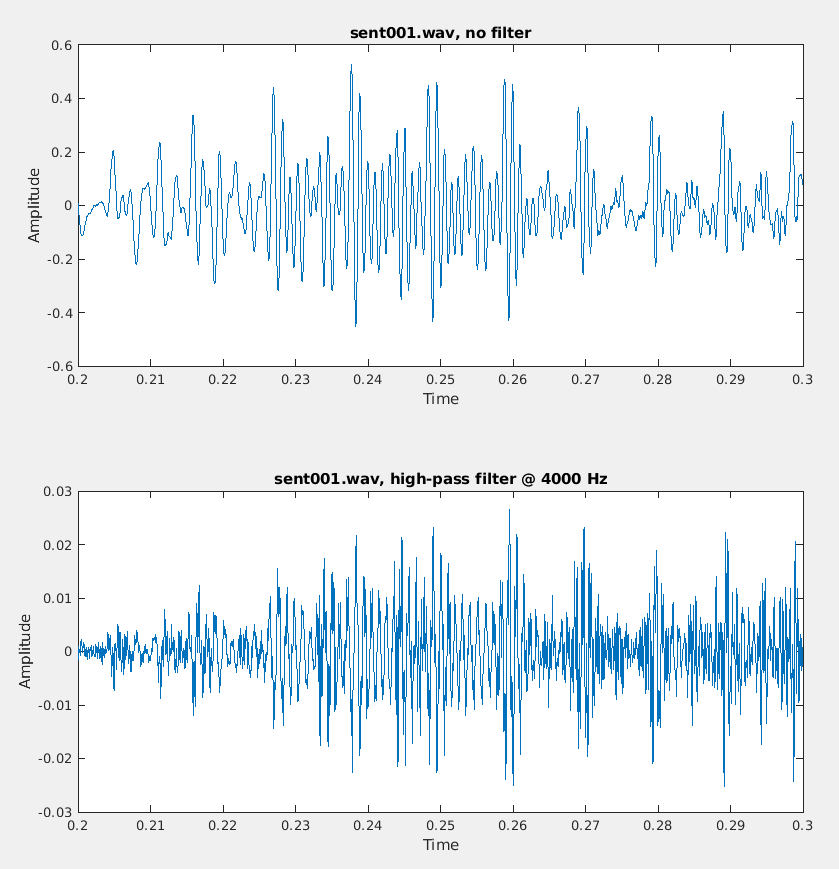
\includegraphics[width=\textwidth]{exercise3.png}

\subsection{Exercise 4}

\lstinputlisting{rectifier_envelope.m}

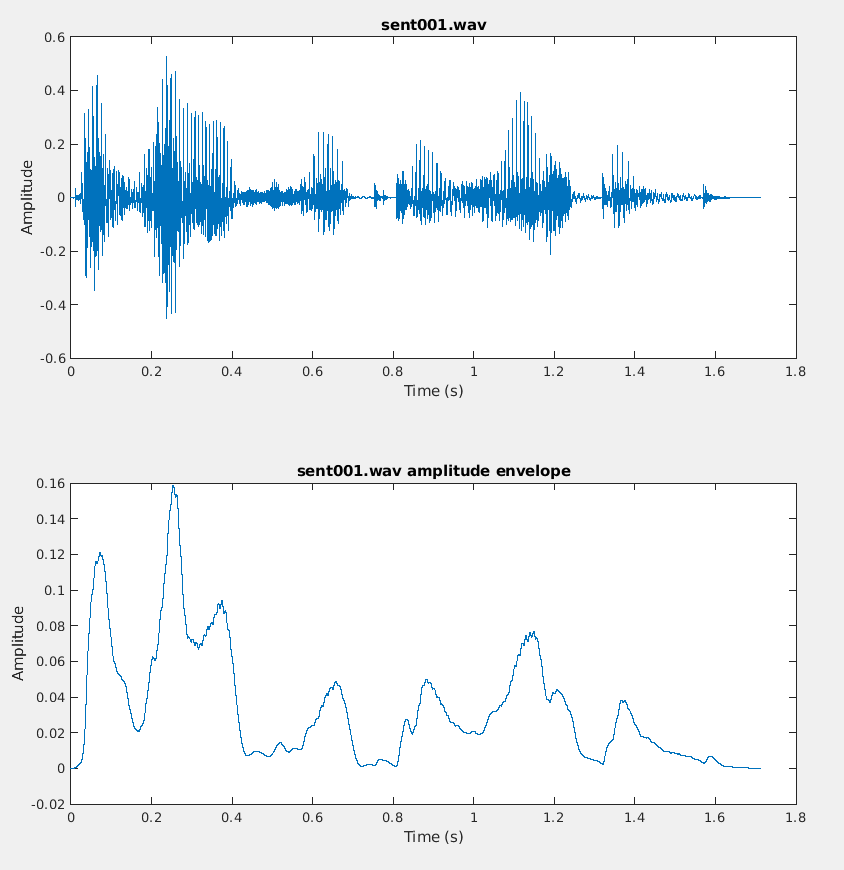
\includegraphics[width=\textwidth]{exercise4.png}

\section{Conclusion}

Within Part 1, Exercise 1 demonstrated the use of \textit{abs()} to create a full rectifier, and \textit{max()} to create a half rectifier.
Exercises 2 and 3 uses \textit{butter()} and the Nyquist frequency to create low-pass and high-pass filters at any given real cutoff frequency.
Exercise 4 composes a full rectifier together with a low-pass filter to extract the envelope from an audio signal.

\end{document}
